\documentclass{article}
\usepackage[utf8]{inputenc}
\usepackage[portuges]{babel}
\usepackage{listings}
\usepackage[table]{xcolor}
\usepackage{verbatim}
\usepackage{indentfirst}
\usepackage{hyperref}
%%\setlength{\parindent}{ex}
\usepackage{graphicx}
\usepackage{fancyhdr}
\usepackage{float}

\title{
       \vspace{60px}
       \Huge \textbf{Serviço de transferência rápida e fiável de dados sobre UDP} \\[15px]
       \Large \textbf{Relatório do trabalho prático}
       %%\vspace{100px}
      }
\author{
        \begin{tabular}{c}
            \textbf{Grupo 9} \\[5px]
                Joana Cruz(A76270) \\
                Etienne Costa (A76089) \\
                Hugo Moreira (A43148)
        \end{tabular}
       }
\date{Maio 2019}

\makeatletter         
\def\@maketitle{
    \begin{center}
        \huge \@title \\[4ex]
        \Large \@author \\[5ex] 
        \@date \\[8px]
        \vspace{100px}
        
\includegraphics[scale=0.40]{img/uminho.png} \\
        \vspace{25px} 
        \small Comunicações por Computador \\[3px]
        Mestrado Integrado em Engenharia Informática \\[3px]
        Universidade do Minho \\
    \end{center}}
\makeatother

\begin{document}
\maketitle

\newpage
\section{Introdução}

Este projeto surge no âmbito da Unidade Curricular de Comunicações por Computador e tem como objetivo a implementação de  um serviço de transferência rápida e fiável de dados sobre UDP. Sendo que a comunicação deverá ser feita em unidades de dados que caibam dentro de um datagrama UDP e que sejam enviados e recebidos via Sockets UDP.
Este serviço de transferência é caracterizado por três fases durante uma conexão: início da conexão, transferência de dados e término da conexão.


\section{Especificação do protocolo}

Sendo um protocolo uma convenção que controla e possibilita uma conexão,comunicação e transferência de dados entre dois sistemas computacionais,dedicou-se está secção para explanar o formato das mensagens protocolares bem com as suas interações.

\subsection{Proposta do PDU}

O serviço de transferência rápida e fiável de dados foi implementado, a nível aplicacional, com recurso ao UDP. Sendo assim houve a necessidade de definir um datagrama UDP  que possui as seguintes características :

\begin{itemize}
    \item \textbf{Sequence Number}:Valor utilizado para garantir a entrega ordenada e robustez durante a transferênca. 
    \item \textbf{Acknowledge}: Valor utilizado para confirmar a entrega de um segmento.
    \item \textbf{Flag Type}: Valores utilizados para indicar um estado particular da conexão ou para fornecer informação adicional.Portanto,
    podem ser usados para fins de solução de problemas ou para controlar como uma determinada conexão é tratada.\\
    De seguida apresenta-se os possíveis valores para estas flags:
    \begin{enumerate}
    \item \textbf{SYN}.
    \item \textbf{ACK}.
    \item \textbf{PSH}
    \item \textbf{SYN+ACK}
    \item \textbf{JOE DOWN}
    \item \textbf{JOE UP}
    \item \textbf{EXIT} 
    \item \textbf{LIST}
    \item \textbf{NOTHING}
    \end{enumerate}
    \item \textbf{Port Number}:
    \item \textbf{Window Size}:Indica em bytes a quantidade de informação que este pode enviar nos próximos pacotes,durante uma conexão.
    \item \textbf{Length Data}: Corresponde em bytes ao tamanho do pacote a ser enviado.
    \item \textbf{CheckSum}: Valor utilizado para verificar a integridade de dados transmititos.
    \item \textbf{File Data}: Corresponde em bytes a informação a ser transferida.
\end{itemize}

\begin{figure}[H]
    \centering
    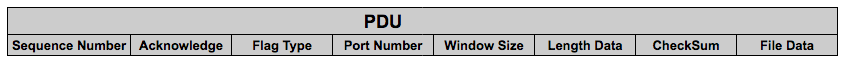
\includegraphics[scale=0.50]{img/pdu.PNG}
    \caption{Protocol Data Unit}
\end{figure}


\subsection{Interação}

O nosso sistema de transferência é caracterizado por três fases distintas durante uma conexão:
\begin{enumerate}
\item \textbf{Início da conexão}
Para o início de uma conexão o nosso sistema foi baseado no 3-Way Handshake do TCP.\\
Sendo que esta conexão procede do seguinte modo:

\begin{table}[h!]
\centering
\begin{tabular}{||c c c c||} 
\hline
\textbf{Início da Conexão} \\ [0.5ex] 
\hline\hline
Host A sends \textbf{SYN}chronize packet to Host B \\ 
Host B receives  \textbf{SYN}  \\
Host B sends  \textbf{SYN}chronize-\textbf{ACK}nowledgment\\
Host A receives  \textbf{SYN-ACK}\\
Host A sends \textbf{ACK}nowledgment \\
Host B receives \textbf{ACK}\\ 
\hline
\end{tabular}
\caption{Início da conexão}
\label{table:1}
\end{table}


\item \textbf{Transferência de Dados}




\item \textbf{Término da conexão}
Para o término de uma conexão ,o nosso sistema foi baseado no TCP,sendo que este término
é um processo de quatro fases, em que cada sistema computacional é responsável pelo encerramento do seu 
lado da ligação.\\

\begin{table}[h!]
\centering
\begin{tabular}{||c c c c||} 
\hline
\textbf{Término da Conexão} \\ [0.5ex] 
\hline\hline
Host A sends a \textbf{FIN}ished packet to Host B \\ 
Host B receives  \textbf{FIN}ished  \\
Host B sends  \textbf{ACK}nowledgment\\
Host A receives \textbf{ACK}nowledgment\\
Host B sends \textbf{FIN}ished packet to Host A \\
Host A receives \textbf{FIN}ished\\
Host A sends  \textbf{ACK}nowledgment\\
Host B receives \textbf{ACK}nowledgment  \\
\hline
\end{tabular}
\caption{Término da conexão}
\label{table:2}
\end{table}
\end{enumerate}


\newpage









\section{Implementação}

\subsection{Arquitetura da solução}

A arquitetura da solução implementada encontra-se descrita na figura apresentada abaixo:

\begin{figure}[H]
    \centering
    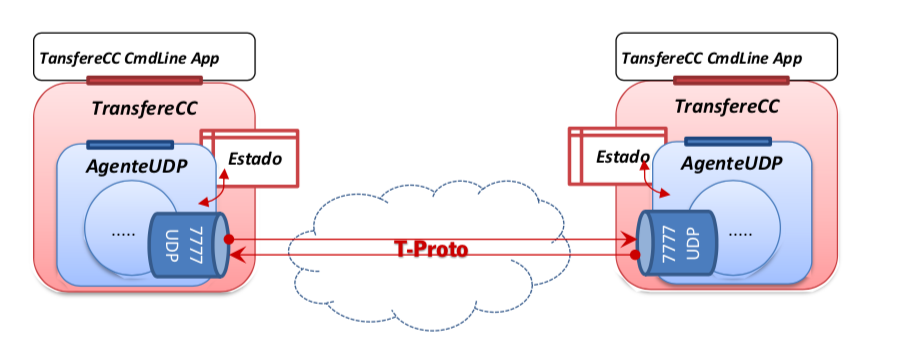
\includegraphics[scale=0.4]{img/arquitetura.PNG}
    \caption{Arquitetura da solução implementada}
\end{figure}


\subsection{Estrutura de dados}

Para a implementação destes conceitos, foi utilizada a linguagem de programação orientada a objectos \emph{Java}, e foram definidas as seguintes classes:
\begin{itemize}
\item \textbf{ClientAgentUDP}:
\item \textbf{ServerAgentUDP}:
\item \textbf{PDU}:
\item \textbf{...}
\item \textbf{...}
\item \textbf{...}
\end{itemize}

\subsection{Métodos}

De modo a não tornar esta leitura exaustiva , decidiu-se simplesmente apresentar os métodos mais relevantes
e procurar explicar o impacto que cada um tem na implementação do nosso serviço.

\begin{enumerate}

\item \textbf{Método da Joaninha de DSS}
\item \textbf{Método da Joaninha do Pintas}
\item \textbf{Método da Grande Líder}

\end{enumerate}

\subsection{Bibliotecas de suporte}

Sendo java uma linguagem de programação bastante versátil foi possível importar todas as bibliotecas que permitissem a realização 
deste projecto,sendo elas as seguintes:

\begin{itemize}
\item{import java.io.IOException;}
\item{import java.net.InetAddress;}
\item{import java.net.SocketException;}
\item{import java.net.UnknownHostException;}
\item{import java.util.concurrent.ConcurrentHashMap;}
\item{import java.util.concurrent.atomic.AtomicBoolean;}
\item{import java.util.logging.Level;}
\item{import java.util.logging.Logger;}
\item{import java.net.SocketException;}
\end{itemize}

\newpage


\section{Funcionalidades Adicionais}


\newpage
\section{Testes e Resultados}


\newpage
\section{Conclusões e trabalho futuro}



\end{document}
